%%%%%%%%%%%%%%%%%%%%%%%%%%%%%%%%%%%%%%%%%%%%%%%%%%%%%%%%%%%%%%%%%%%%%%%%
% Plantilla TFG/TFM
% Escuela Politécnica Superior de la Universidad de Alicante
% Realizado por: Jose Manuel Requena Plens
% Contacto: info@jmrplens.com / Telegram:@jmrplens
%%%%%%%%%%%%%%%%%%%%%%%%%%%%%%%%%%%%%%%%%%%%%%%%%%%%%%%%%%%%%%%%%%%%%%%%

\chapter{Resultados}
\label{resultados}



  En esta sección se detallarán los resultados de los experimentos y se realizará un análisis comparativo entre ellos.


  En primer lugar....

\section{Algoritmo Genético}

  En la figura [\ref{EvolucionHiperparametrosImage}] se pueden visualizar la evolución de los parámetros del mejor individuo en cada generación.

  \begin{figure}[H]
      \centering
      \includesvg[scale=0.4]{archivos/5.Resultados/GA/EvolucionHiperparametros}
      \caption{Evolución de hiperparámetros a lo largo de las iteraciones.}
      \label{EvolucionHiperparametrosImage}
   \end{figure}

  \begin{figure}[H]
      \centering
      \includesvg[scale=0.4]{archivos/5.Resultados/GA/EvolucionF1Score}
      \caption{Evolución del macro F1 score a lo largo de las iteraciones.}
      \label{EvolucionF1ScoreImage}
   \end{figure}

  En la tabla \ref{BestGASolutionTable} se pueden observar el mejor individuo obtenido después de \textit{TODO: X} generaciones.

  \begin{table}[H]
      \centering
          \begin{tabular}{ |c|c| } 
              \hline
              \textbf{Hiperparámetro} & \textbf{Valor}\\
              \hline
                  Profundidad Máxima & TODO \\ 
                  Peso mínimo de los hijos & TODO \\ 
                  ETA & TODO \\ 
              \hline

          \end{tabular}
      \caption{Mejores parámetros de XGBoost tras aplicar el algoritmo genético.}
      \label{BestGASolutionTable}
  \end{table}

\section{XGBoost}

  \begin{figure}[H]
      \centering
      \includesvg[scale = 0.6]{archivos/5.Resultados/XGBoost/FeatureWeights}
      \caption{Pesos asignados por XGboost a las características.}
      \label{FeatureWeightsImage}
   \end{figure}

\section{KNN}
  Se puede observar en la tabla \ref{BestParamsKNNGridSearchTable} los mejores parámetros para \textit{KNN} después de haber ejecutado \textit{Grid Search} sobre el conjunto de entrenamiento.\\

  \begin{table}[H]
      \centering
      \begin{tabular}{ |c|c| }
          \hline
          Atributo & Valor\\
          \hline
              Número de vecinos & 91 \\ 
              Tipo de distancia & Minkowski \\ 
          \hline
      \end{tabular}
      \caption{Mejores parámetros de KNN tras aplicar GridSearch.}
      \label{BestParamsKNNGridSearchTable}
  \end{table}


  \begin{table}[H]
    \centering
    \begin{tabular}{ |c|c|c|c| }
         \hline
         \textbf{Categoría} & \textbf{Peso Categoría} & \textbf{Característica} & \textbf{Peso Característica}\\

         \hline
         \multirow{4}{*}{Accidente}   & \multirow{4}{*}{TODO: 1}      & Coordenada X          & TODO: 1\\
                                      &                               & Coordenada Y          & TODO: 1\\
                                      &                               & Hora                  & TODO: 1\\
                                      &                               & Vehículos implicados  & TODO: 1\\

         \hline
         \multirow{1}{*}{Ambiente}    & \multirow{1}{*}{TODO: 1}      & Estado meteorológico  & TODO: 1\\

         \hline
         \multirow{2}{*}{Carretera}   & \multirow{2}{*}{TODO: 1}      & Tipo de accidente     & TODO: 1\\
                                      &                               & Distrito              & TODO: 1\\

         \hline
         \multirow{4}{*}{Conductor}   & \multirow{4}{*}{TODO: 1}      & Tipo Persona          & TODO: 1\\
                                      &                               & Sexo                  & TODO: 1\\
                                      &                               & Rango Edad            & TODO: 1\\
                                      &                               & Positivo              & TODO: 1\\
         \hline
    \end{tabular}

    \caption{Cálculo de pesos de características y categorías mediante XGBoost.}
    \label{PesosFinalesCaracteristicas}
  \end{table}


  El resultado de aplicar ambas técnicas da lugar a la representación en forma matricial de los accidentes, como se puede observar en la figura \ref{SampledImagesExampleImage}.

\section{Entrenamiento de modelos}

  \subsection{Tiempos de entrenamiento}

    \textbf{El KNN no necesita entrenamiento, el tiempo obtenido es el de la optimización de hiperparámetros mediante Grid Search, por lo que no incluiría el tiempo en la gráfica.}

    \begin{figure}[h]
      \centering
      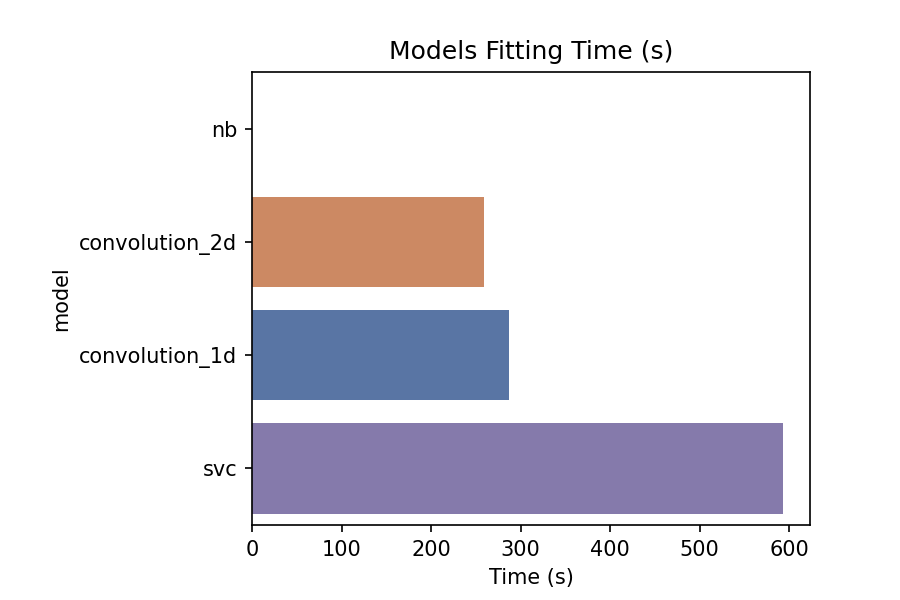
\includegraphics[width=16cm]{archivos/5.Resultados/TiemposEntrenamiento}
      \caption{Comparación entre los tiempos de entrenamiento de los modelos.}
      \label{TiemposEntrenamientoImage}
    \end{figure}

  
  \subsection{Gráficas de entrenamiento}

    Explicar las gráficas de evolución F1-score de las redes neuronales.


    \begin{figure}[h]
        \centering
        \includesvg[scale=0.3]{archivos/5.Resultados/CNN/1D/F1Score1D}
        \caption{Comparación de TODO(tipo) F1 score sobre el conjunto de entrenamiento y validación CNN-1D.}
        \label{F1Score1DImage}
     \end{figure}


    \begin{figure}[h]
        \centering
        \includesvg[scale=0.3]{archivos/5.Resultados/CNN/2D/F1Score2D}
        \caption{Comparación de TODO(tipo) F1 score sobre el conjunto de entrenamiento y validación CNN-2D.}
        \label{F1Score2DImage}
     \end{figure}


  \subsection{Reportes de clasificación}
       
    Explicar los reportes de clasificación con datos de \textbf{ENTRENAMIENTO.}

    \begin{table}
        \scriptsize

        \begin{subtable}{.2\textwidth}
          \renewcommand{\arraystretch}{1.2}

          \csvautotabular{archivos/5.Resultados/CNN/1D/1DClassificationReportTrain.csv}
          \caption{Métricas de clasificación del conjunto de entrenamiento CNN-1D.}
          \label{CNN1DMetrics}
        \end{subtable}
        \hspace{17em}
        \begin{subtable}{.2\textwidth}
          \renewcommand{\arraystretch}{1.2}

          \csvautotabular{archivos/5.Resultados/NB/NBClassificationReportTrain.csv}
          \caption{Métricas clasificación del conjunto de entrenamiento Naive Bayes.}
          \label{NBMetrics}
        \end{subtable}
        \vskip\baselineskip

        \begin{subtable}{.2\textwidth}
          \centering
          \renewcommand{\arraystretch}{1.2}

          \csvautotabular{archivos/5.Resultados/SVC/SVCClassificationReportTrain.csv}
          \caption{Métricas clasificación del conjunto de entrenamiento SVC.}
          \label{SVCDMetrics}
        \end{subtable}
        \hspace{17em}
        \begin{subtable}{.2\textwidth}
          \renewcommand{\arraystretch}{1.2}

          \csvautotabular{archivos/5.Resultados/KNN/KNNClassificationReportTrain.csv}
          \caption{Métricas clasificación del conjunto de entrenamiento KNN.}
          \label{KNNMetrics}
        \end{subtable}

        \begin{subtable}{.2\textwidth}
          \centering
          \renewcommand{\arraystretch}{1.2}

          \csvautotabular{archivos/5.Resultados/CNN/2D/2DClassificationReportTrain.csv}
          \caption{Métricas clasificación del conjunto de entrenamiento CNN-2D.}
          \label{CNN2DMetrics}
        \end{subtable}
    \end{table}

  \subsection{Matrices de confusión}

    Explicar las matrices de confusión con datos de \textbf{ENTRENAMIENTO.}

    \begin{figure}
        \centering
        \begin{subfigure}[b]{0.4\textwidth}
            \centering
            \includesvg[scale=0.4]{archivos/5.Resultados/CNN/1D/1DConfusionMatrixTrain}
            \caption{Matriz de confusión sobre el conjunto de datos de entrenamiento CNN-1D.}
            \label{ConfusionMatrixTrainImages:1D}
        \end{subfigure}
        % Añadir el espacio deseado, si se deja la linea en blanco la siguiente subfigura ira en una nueva linea
        \begin{subfigure}[b]{0.4\textwidth}
            \centering
            \includesvg[scale=0.4]{archivos/5.Resultados/CNN/2D/2DConfusionMatrixTrain}
            \caption{Matriz de confusión sobre el conjunto de datos de entrenamiento CNN-2D.} 
            \label{ConfusionMatrixTrainImages:2D}

        \end{subfigure}
        \begin{subfigure}[b]{0.4\textwidth}
            \centering
            \includesvg[scale=0.4]{archivos/5.Resultados/NB/NBConfusionMatrixTrain}
            \caption{Matriz de confusión sobre el conjunto de datos de entrenamiento NB.}
            \label{ConfusionMatrixTrainImages:NB}
        \end{subfigure}

        \begin{subfigure}[b]{0.4\textwidth}
            \centering
            \includesvg[scale=0.4]{archivos/5.Resultados/KNN/KNNConfusionMatrixTrain}
            \caption{Matriz de confusión sobre el conjunto de datos de entrenamiento KNN.}
            \label{ConfusionMatrixTrainImages:KNN}
        \end{subfigure}

        \begin{subfigure}[b]{0.4\textwidth}
            \centering
            \includesvg[scale=0.4]{archivos/5.Resultados/SVC/SVCConfusionMatrixTrain}
            \caption{Matriz de confusión sobre el conjunto de datos de entrenamiento SVC.}
            \label{ConfusionMatrixTrainImages:SVC}
        \end{subfigure}

        \caption{Matrices de confusión de los modelos sobre el conjunto de entrenamiento.}
        \label{ConfusionMatrixTrainImages}
     \end{figure}

  \subsection{Comparativa entre modelos}

    Explicar la comparativa de modelos con datos de \textbf{ENTRENAMIENTO.}


    \begin{figure}[h]
        \centering
        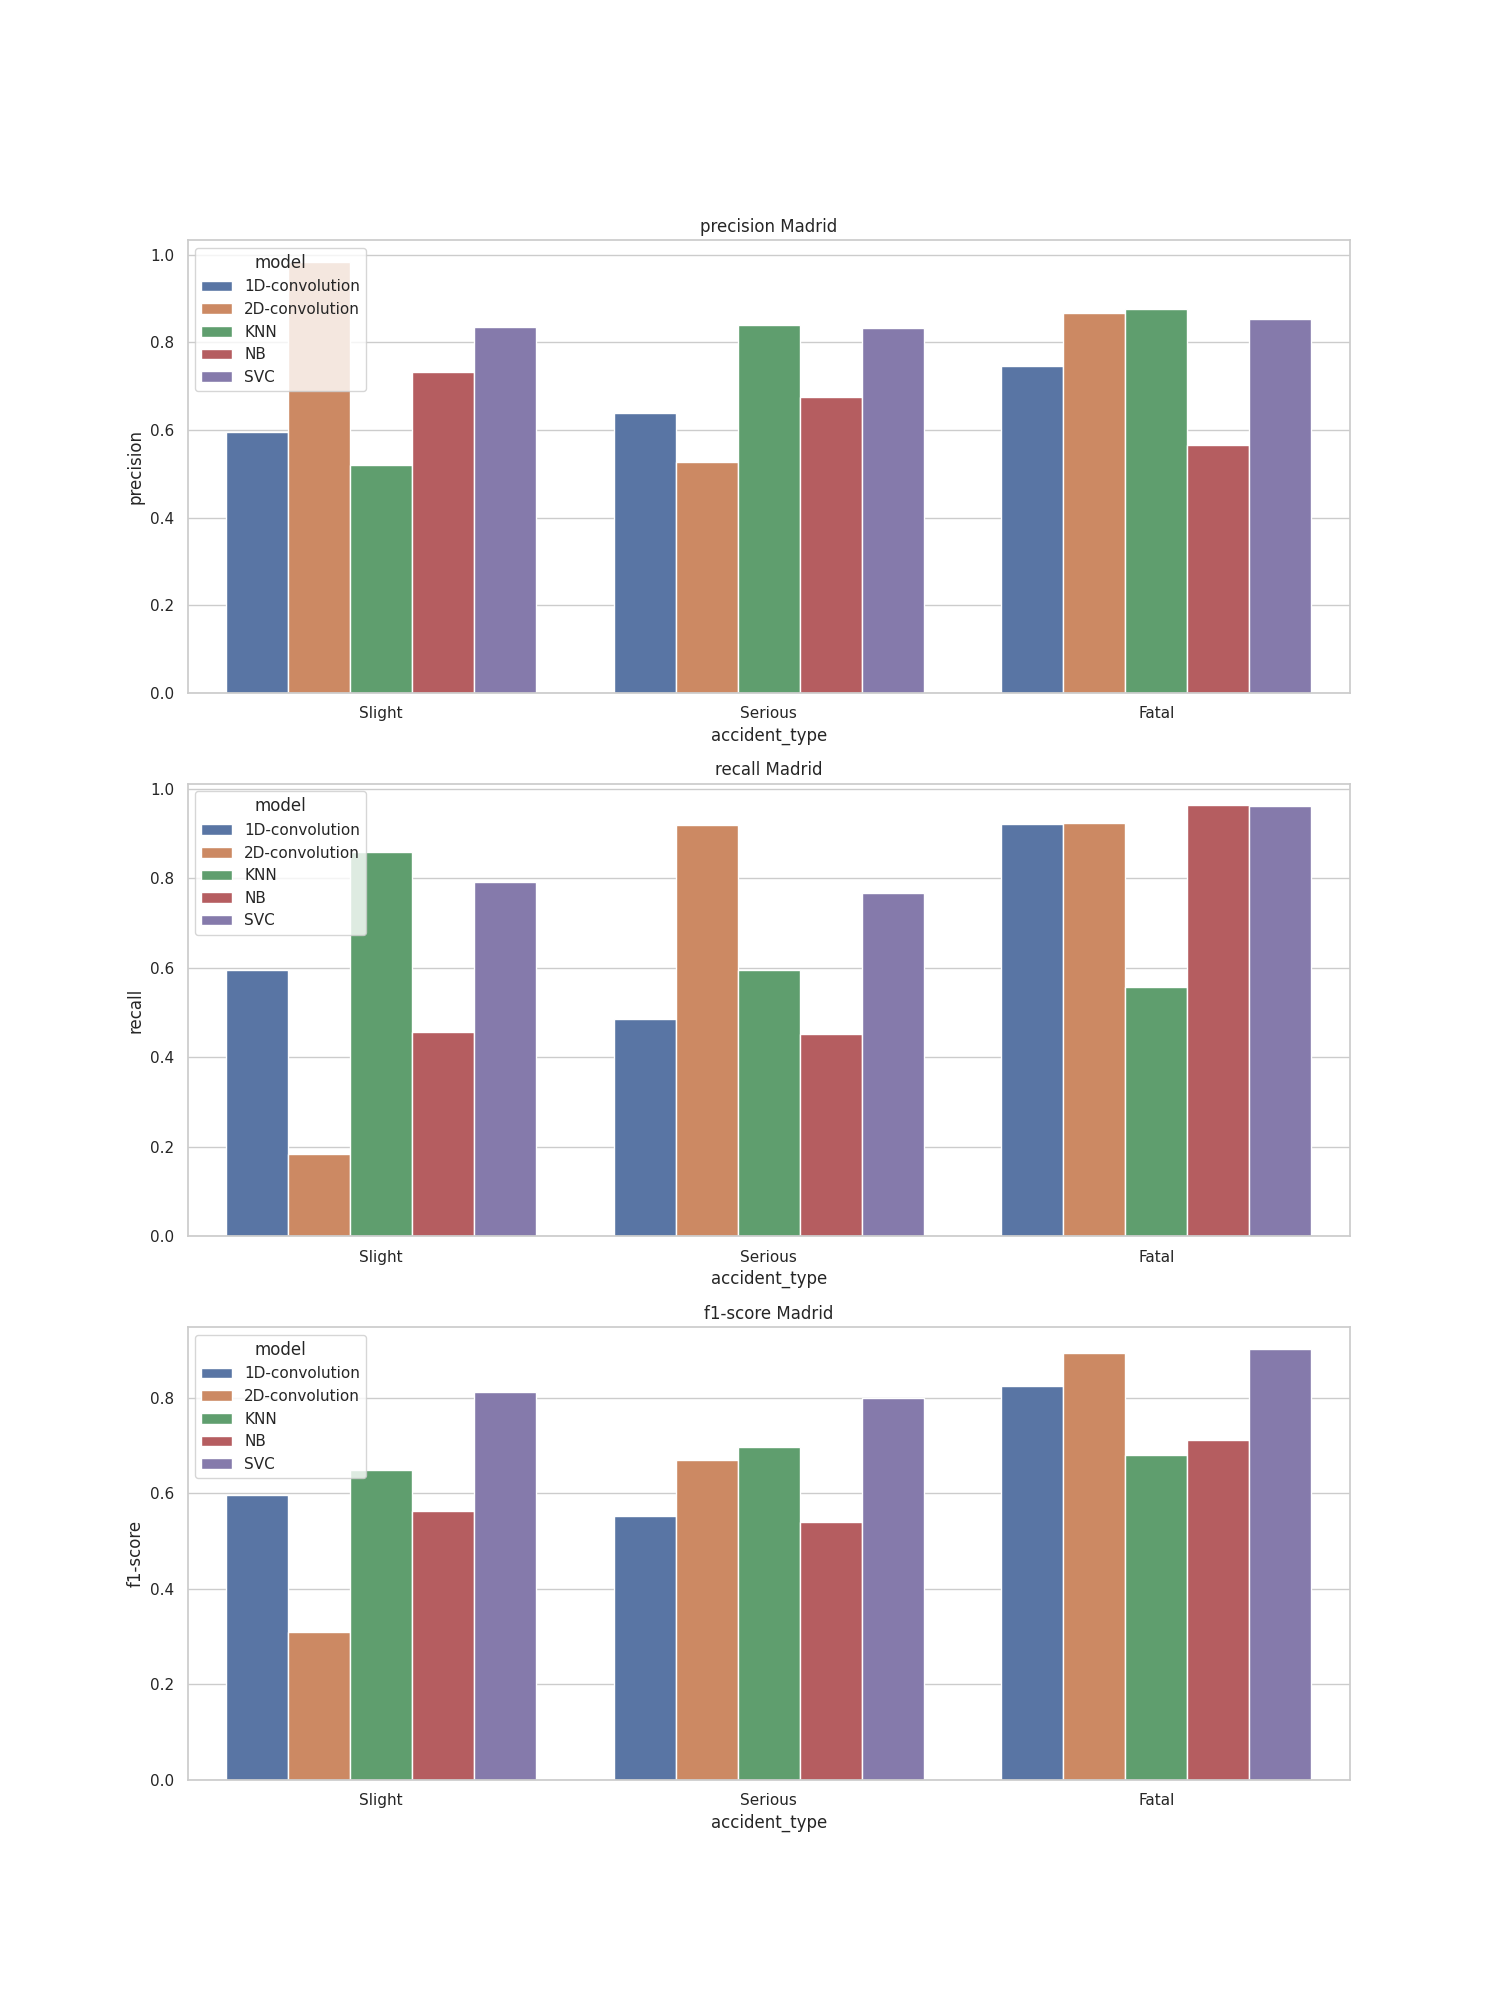
\includegraphics[width=16cm]{archivos/5.Resultados/ComparativaTrain}
        \caption{Comparativa de las métricas de las predicciones sobre el conjunto de entrenamiento de los modelos.}
        \label{ResultsTrainImage}
     \end{figure}



\section{Predicciones de modelos}

  \subsection{Reportes de clasificación}

    Explicar los reportes de clasificación con datos de \textbf{TEST.}

    \begin{table}[H]
      \centering
      \csvautotabular{archivos/5.Resultados/CNN/1D/1DClassificationReportTest.csv}
      \caption{Métricas CNN-1D.}
      \label{CNN1DMetrics}
    \end{table}

    \begin{table}[H]
      \centering
      \csvautotabular{archivos/5.Resultados/NB/NBClassificationReportTest.csv}
      \caption{Métricas Naive Bayes.}
      \label{NBMetrics}
    \end{table}

    \begin{table}[H]
      \centering
      \csvautotabular{archivos/5.Resultados/SVC/SVCClassificationReportTest.csv}
      \caption{Métricas SVC.}
      \label{SVCDMetrics}
    \end{table}

    \begin{table}[H]
      \centering
      \csvautotabular{archivos/5.Resultados/KNN/KNNClassificationReportTest.csv}
      \caption{Métricas SVC.}
      \label{SVCDMetrics}
    \end{table}

    \begin{table}[H]
      \centering
      \csvautotabular{archivos/5.Resultados/CNN/2D/2DClassificationReportTest.csv}
      \caption{Métricas CNN-2D.}
      \label{CNN2DMetrics}
    \end{table}

  \subsection{Matrices de confusión}

    Explicar las matrices de confusión con datos de \textbf{TEST.}


    \begin{figure*}
        \centering
        \begin{subfigure}[b]{0.4\textwidth}
            \centering
            \includesvg[scale=0.4]{archivos/5.Resultados/CNN/1D/1DConfusionMatrixTest}
            \caption{Matriz de confusión CNN-1D.}
            \label{ConfusionMatrixTestImages:1D}
        \end{subfigure}
        \hspace{3em}
        % Añadir el espacio deseado, si se deja la linea en blanco la siguiente subfigura ira en una nueva linea
        \begin{subfigure}[b]{0.4\textwidth}
            \centering
            \includesvg[scale=0.4]{archivos/5.Resultados/CNN/2D/2DConfusionMatrixTest}
            \caption{Matriz de confusión CNN-2D.} 
            \label{ConfusionMatrixTestImages:2D}

        \end{subfigure}
        \vskip\baselineskip
        \begin{subfigure}[b]{0.4\textwidth}
            \centering
            \includesvg[scale=0.4]{archivos/5.Resultados/NB/NBConfusionMatrixTest}
            \caption{Matriz de confusión NB.}
            \label{ConfusionMatrixTestImages:NB}
        \end{subfigure}
        \hspace{3em}
        \begin{subfigure}[b]{0.4\textwidth}
            \centering
            \includesvg[scale=0.4]{archivos/5.Resultados/KNN/KNNConfusionMatrixTest}
            \caption{Matriz de confusión KNN.}
            \label{ConfusionMatrixTestImages:KNN}
        \end{subfigure}
        \vskip\baselineskip
        \begin{subfigure}[b]{0.4\textwidth}
            \centering
            \includesvg[scale=0.4]{archivos/5.Resultados/SVC/SVCConfusionMatrixTest}
            \caption{Matriz de confusión SVC.}
            \label{ConfusionMatrixTestImages:SVC}
        \end{subfigure}

        \caption{Matrices de confusión de los modelos sobre el conjunto de entrenamiento.}
        \label{ConfusionMatrixTestImages}
     \end{figure*}

  \subsection{Comparativa entre modelos}

    Explicar la comparativa de modelos con datos de \textbf{ENTRENAMIENTO.}


    \begin{figure}[h]
        \centering
        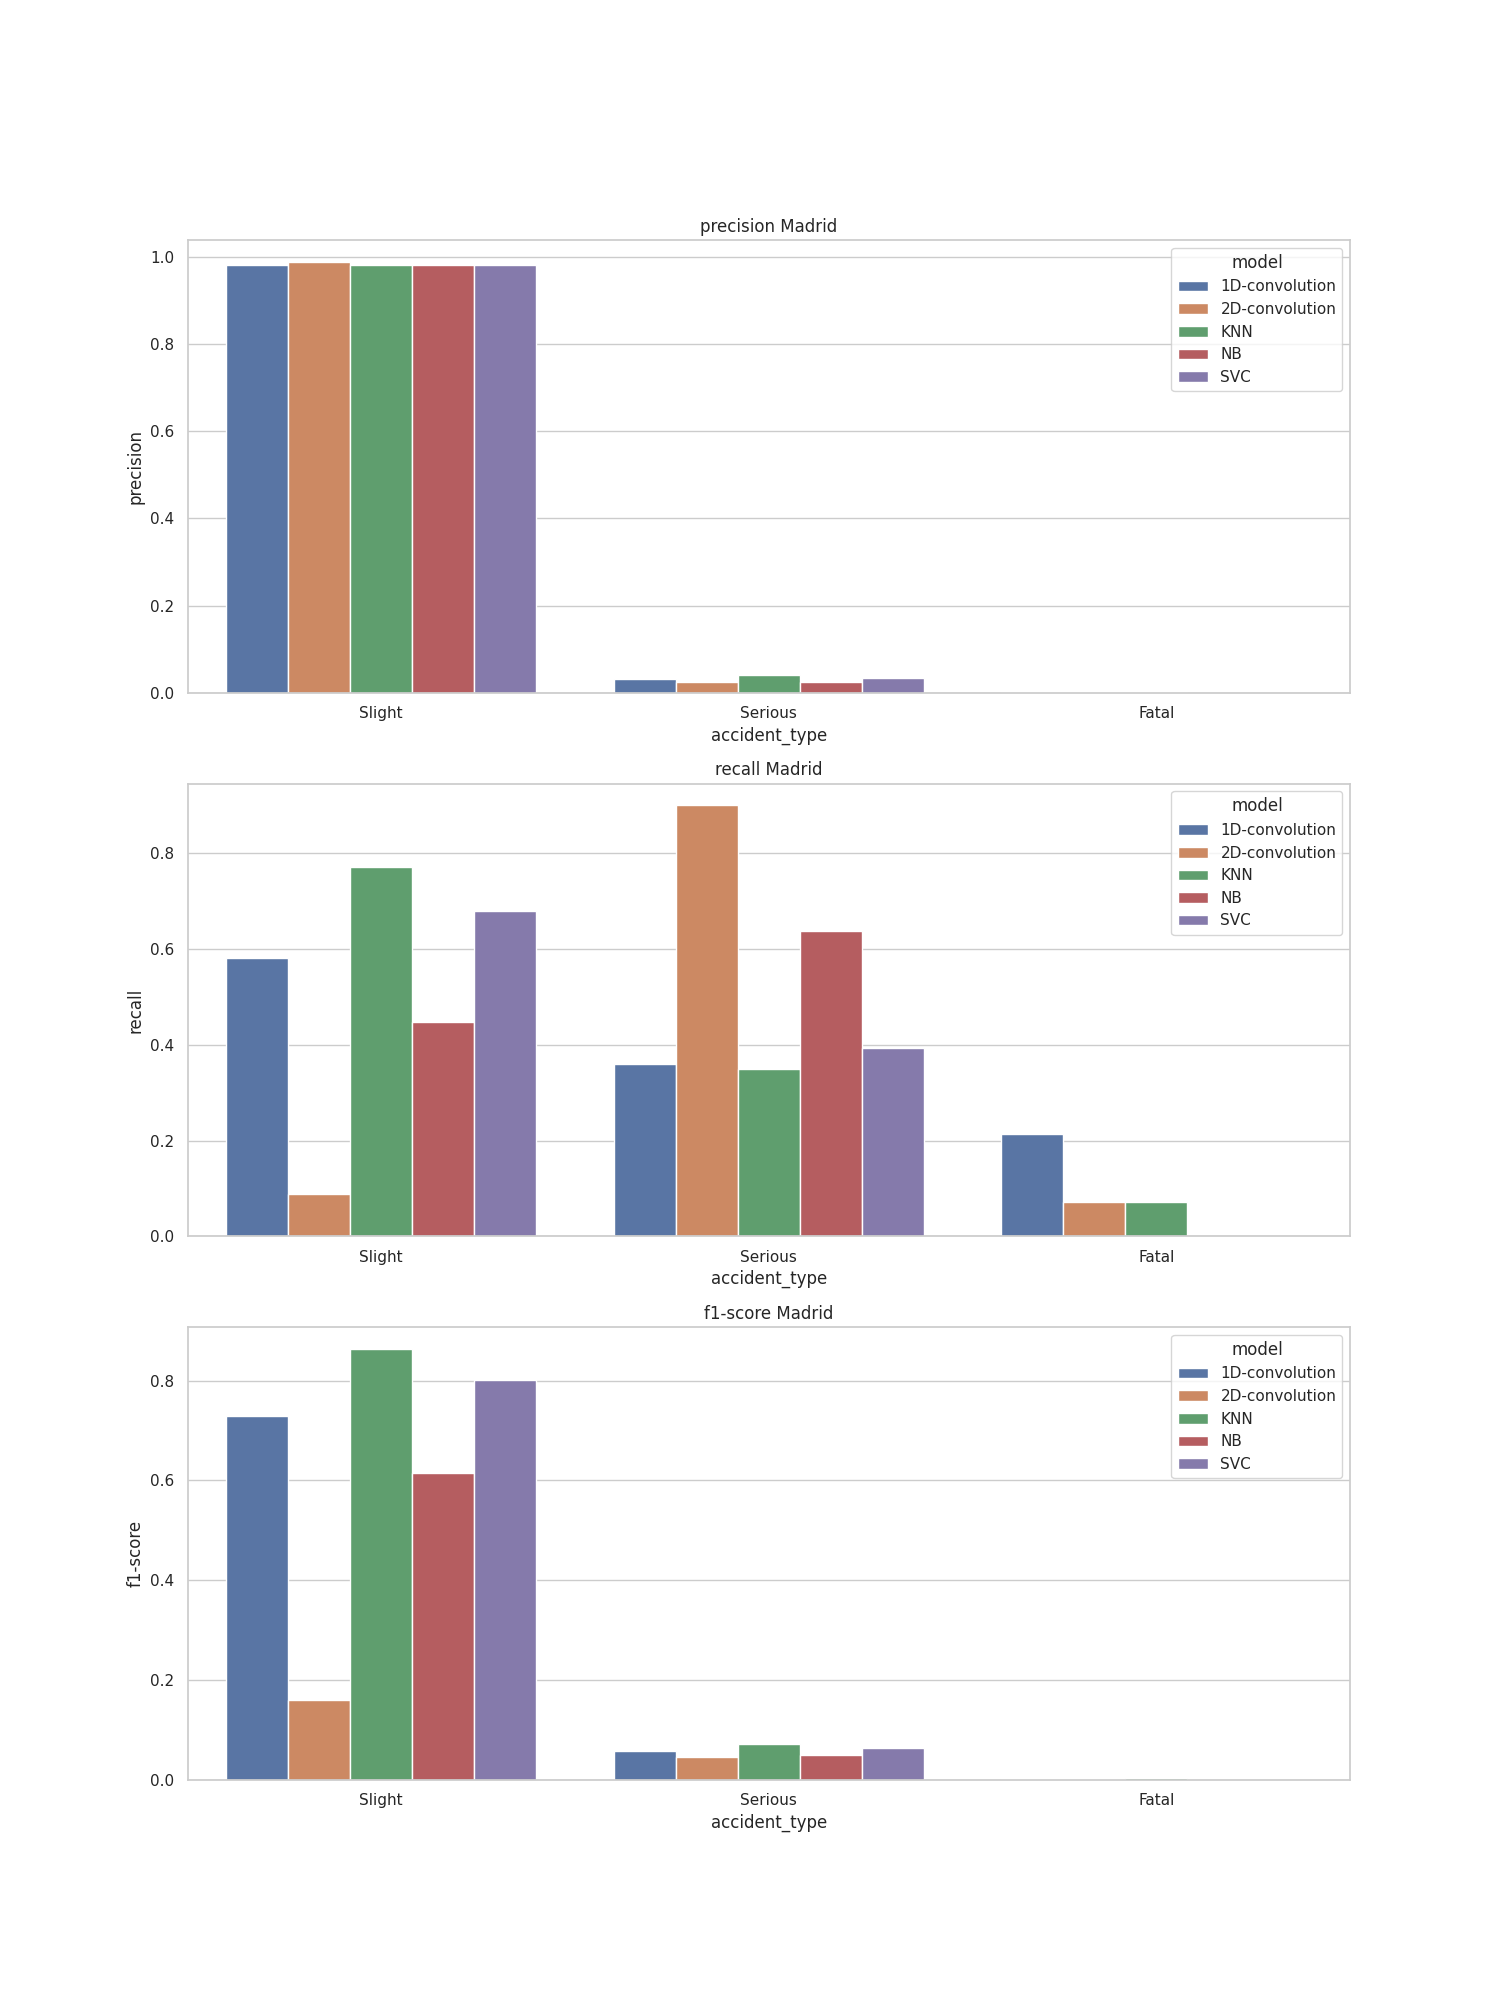
\includegraphics[width=16cm]{archivos/5.Resultados/ComparativaTest}
        \caption{Comparativa de las métricas de las predicciones sobre el conjunto de test de los modelos.}
        \label{ResultsTestImage}
     \end{figure}



Como podemos observar, los modelos entrenados predicen bien sus muestras de enrenamiento sin embargo inguno de los modelos aplicados es capaz de generalizar bien sore el conjunto de datos de test sin smote
esto es debido a la naturaleza de los datos, de la informacio que tenemos y de el tipo de limpieza que se ha hecho. Se ppodria hacer un estudio del valor numerico que se le asigna a cada variable en la limpieza, ya que seguramente al estar nosotros haciendolo aleatoriamente seguramente se esté creando algún patrón de jerarquía dentro de una columna o se le da mas importancia a un todoterreno que a un avion porque el todoterrento al tener un valor asignado más alto sera mas negro y por lo tanto la red predicira lo que sea